\documentclass[10pt,letterpaper]{article}

\usepackage[margin=1in]{geometry}
\usepackage{microtype}
\usepackage{booktabs}
\usepackage{graphicx}
\usepackage{caption}
\usepackage{subcaption}
\usepackage{xcolor}
\usepackage[hidelinks]{hyperref}
\usepackage[round]{natbib}
\usepackage{titlesec}

% Tighter section spacing
\titlespacing*{\section}{0pt}{12pt}{4pt}
\titlespacing*{\subsection}{0pt}{8pt}{2pt}

% Tighter caption spacing
\captionsetup{font=small, labelfont=bf, skip=4pt}

\title{\bfseries Five Methodological Tiers of Entity Resolution: \\
A Comparative Study Across Four Benchmark Datasets\thanks{Work
performed at Johns Hopkins University in Spring 2023 (course
EN.601.507, advised by Dr.\ Tom Lippincott).}}

\author{Johnny Saldana \\
Johns Hopkins University \\
\texttt{johnny.saldana99@gmail.com}}

\date{}

\begin{document}

\maketitle

\begin{abstract}
\noindent
Entity resolution is the problem of deciding whether two records refer
to the same real-world entity. It sits at the foundation of data
integration, master-data management, and any analytical workflow that
draws on more than one source. We present \texttt{matchify}, a
reproducible Python package that implements five entity-resolution
models spanning the methodological progression of the field, from a
hash-based exact-match baseline to a fine-tuned twin-encoder Siamese
network. The five models are exposed under a single abstract interface
and evaluated on four benchmark datasets (Amazon-Google Products,
Abt-Buy, DBLP-ACM, and a controlled synthetic person-record corpus).
Our contribution is threefold. We provide a reproducible reference
implementation of five entity-resolution methods under a unified
interface. We adopt a held-out group-split evaluation protocol that
prevents the supervision leakage common in older entity-resolution
evaluations, in which test-row group identifiers were sometimes
visible to the supervised classifiers at training time. And we report
an empirical observation that engineered distance-feature classifiers
still outperform pretrained encoders, with or without fine-tuning, on
small-vocabulary cross-catalog product data. Mean reciprocal rank and
threshold-swept precision-recall curves with multi-seed standard
deviations on the stochastic models support the finding. On the
Abt-Buy benchmark a supervised multilayer perceptron over engineered
field similarities outperforms both pretrained sentence-BERT and a
fine-tuned Siamese variant by a wide margin, suggesting that on
small-vocabulary, high-variance product corpora, the choice of feature
representation still dominates the choice of architecture.

\medskip
\noindent\textbf{Code and data.}
\url{https://github.com/johnnysaldana/matchify}
\end{abstract}

\section{Introduction}

Most modern data integration pipelines combine sources that lack
unique entity identifiers \citep{christen2012}. The result is a record
linkage problem at scale. Every workflow that combines census tables,
hospital records, customer databases, or e-commerce catalogs must
decide which records refer to the same real-world entity. The problem
appears under several names in the literature, including record
linkage, deduplication, object identification, and entity matching. We
use the term entity resolution following the survey of
\citet{papadakis2021}.

The field has been studied for more than half a century, beginning
with the probabilistic record linkage formalism of
\citet{fellegi1969}. It has since absorbed advances from string
similarity, machine learning, distributed systems, crowd computation,
and most recently deep learning. \citet{christen2012} provides the
canonical textbook treatment. \citet{papadakis2021} organize the
entire history into four generations, characterized by the dominant
paradigm of each era. \citet{binette2022} review the modern
probabilistic and Bayesian methods that have grown out of the
Fellegi-Sunter framework.

Despite this history the field continues to evolve. \citet{mudgal2018}
demonstrate that a deep learning architecture they call DeepMatcher
outperforms classical rule-based systems on a range of benchmarks.
\citet{ebraheem2018} introduce DeepER, a deep representation learning
approach to entity resolution built on distributed tuple
representations. \citet{li2020} extend the deep line by fine-tuning
pretrained transformer language models, achieving state-of-the-art F1
on every standard benchmark. Yet the underlying problem has not
changed, and the choice of method for any given dataset remains a
question of judgment.

This paper presents \texttt{matchify}, a Python package that
implements five entity resolution models under a single abstract
interface and evaluates them on four benchmark datasets under a
consistent experimental protocol. The five models trace the
methodological progression of the field. The first is a hash-based
exact-match baseline that establishes a lower bound for any
non-trivial method.
The second is a configurable rule-based field-similarity model in the
spirit of the Magellan toolkit \citep{konda2016}, supporting per-field
type-aware normalization, four string-similarity metrics, and four
blocking strategies. The third is a supervised multilayer perceptron
trained on sampled positive and negative pairs, with each pair
represented as a fixed-length vector of per-field similarity scores.
The fourth uses a pretrained sentence-transformer
\citep{reimers2019} without fine-tuning, ranking candidate records by
cosine similarity in the encoder's output space. The fifth fine-tunes
the same encoder under a contrastive objective \citep{hadsell2006}.
The twin-encoder Siamese configuration for entity resolution is
studied in detail by \citet{ebraheem2018}, who introduce a related
deep representation learning approach called DeepER.

The contribution of this paper is not a novel method. Each of the five
models is well-grounded in prior work. The contribution is a
reproducible reference implementation under a single interface, a
disciplined evaluation protocol that holds out groups rather than
individual records, and a discussion of where the empirical results
align with the expectations the literature would set and where they
diverge. The full code, data, and trained model artifacts are
available at the package repository.

The remainder of the paper is organized as follows. Section
\ref{sec:background} surveys the relevant background and prior work.
Section \ref{sec:models} describes the five models in detail, with
citations to the methodological line each draws on. Section
\ref{sec:datasets} introduces the four benchmark datasets. Section
\ref{sec:protocol} specifies the evaluation protocol. Section
\ref{sec:results} reports the results. Section \ref{sec:discussion}
discusses where the findings align with expectations and where they
do not. Section \ref{sec:baselines} compares against published F1
numbers from DeepMatcher and Ditto. Section \ref{sec:limitations}
acknowledges limitations. Section \ref{sec:reproducibility} documents
reproducibility.

\section{Background and Related Work}
\label{sec:background}

\subsection{Definitions}

Following \citet{christen2012}, let A and B be two databases of
records described over the same or partially overlapping schemas. The
entity resolution task is to determine, for every pair of records (a,
b) with a in A and b in B, whether the two records refer to the same
real-world entity. A binary decision suffices for many applications,
but more general formulations \citep{binette2022} ask for a clustering
of all records, a probability of being a match, or a ranked list of
candidate matches per query record. The package described here
implements the ranked-list formulation primarily and derives binary
classification at any chosen threshold from those rankings.

\subsection{Generations of entity resolution}

\citet{papadakis2021} organize the field into four generations. The
first is the probabilistic linkage tradition of \citet{fellegi1969},
in which the match decision is grounded in a likelihood ratio of the
observed pair under a match hypothesis versus a non-match hypothesis.
The second generation introduces approximate string similarity and
rule-based decision systems. \citet{bilenko2003} study
string-similarity functions adapted to the matching task.
\citet{cohen2003} provide a comparative empirical study of string
distances. \citet{benjelloun2009} generalize rule-based matching to a
generic algebraic framework called Swoosh, treating match and merge
functions as black boxes whose properties (idempotence, commutativity,
associativity, representativity) determine which efficient algorithm
applies. The third generation incorporates supervised machine
learning, blocking, and parallel execution. \citet{konda2016} describe
Magellan, a toolkit that supports blocking, sampling, labeling,
supervised pair classification, and quality debugging.
\citet{wang2012} introduce CrowdER, which delegates the most uncertain
pairs to crowd workers under a hybrid human-in-the-loop scheme.
\citet{bahmani2017} describe ERBlox, a hybrid that combines matching
dependencies with classifier-based duplicate detection. The fourth
generation is the deep learning era. \citet{mudgal2018} introduce
DeepMatcher and study a design space of attribute encoders, attention
mechanisms, and hybrid combinations. \citet{ebraheem2018} introduce
DeepER, which uses distributed tuple representations built on word
embeddings combined with LSTM-based similarity composition.
\citet{li2020} extend the line with Ditto, a fine-tuned transformer
that establishes new state of the art across multiple benchmarks. The
five models in \texttt{matchify} correspond, roughly, to generations
one through four of this taxonomy.

\subsection{Blocking}

For a database of N records, a naive comparison of every pair scales
quadratically and is intractable beyond a few thousand records. The
standard remedy is blocking, also called indexing, in which a cheap
keying function partitions the database so that comparisons need only
be performed within blocks. \citet{christen2012} catalogs the standard
blocking strategies, including standard equality blocking, sorted
neighborhood, q-gram blocking, and canopy clustering. The package
supports prefix blocking, sorted neighborhood, equality blocking, and
a no-block ``full'' mode for small datasets. Blocking choice is part
of the model configuration in all five tiers.

\subsection{Evaluation}

\citet{papadakis2021} note that ER evaluation is conducted with two
families of metrics. The classification family includes precision,
recall, and F1 over the set of all candidate pairs that the model
produces. The ranking family includes mean reciprocal rank (MRR), mean
average precision, and recall at k. A practitioner who needs a final
yes-or-no decision will typically use F1 at a chosen threshold. A
practitioner who needs ranked candidate lists for downstream review
will use MRR. The evaluation in this paper reports both, with the
recognition that the two metrics measure different things.

The protocol caveat that we discuss in Section \ref{sec:baselines} is
that classification F1 reported in the deep ER literature
\citep[e.g.,][]{mudgal2018, li2020} is computed on a labeled-pair test
set, that is, a set of pairs sampled from the perfect mapping, and not
on the all-pairs candidate set produced by blocking. This makes their
numbers an upper bound on what is achievable rather than a direct
head-to-head comparison.

\section{Models}
\label{sec:models}

\subsection{ExactMatchModel}

The first model is a hash-based exact-match baseline. For each record
r in the input table, we compute the hash of the tuple of all
non-ignored fields. Two records are predicted to refer to the same
entity if and only if they have the same hash. There is no training
phase, no blocking step, and no notion of partial similarity.

This baseline is included for two reasons. The first is to establish
a lower bound on what any nontrivial method should beat. The second is
to surface datasets in which exact duplication is sufficient. Section
\ref{sec:results} shows that on the controlled synthetic person
dataset, where 20\% of the records are perfect duplicates by
construction, the exact-match baseline achieves recall 0.41 and
precision 1.0 at threshold 0.5.

\subsection{FlexMatchModel}

The second model is a configurable rule-based field-similarity model
in the spirit of Magellan \citep{konda2016}. For each pair of records
the model computes a normalized similarity score per field, sums those
scores into a single record-level score, and ranks candidates by that
score. Each field is associated with a type that selects an
appropriate normalizer, drawing on the type-aware preprocessing
strategies catalogued by \citet[chap.\ 3]{christen2012}. Names are
parsed and lowercased. Phone numbers are normalized to E.164 format
with a US default region. Addresses are parsed and lowercased. Dates
are parsed and serialized as ISO 8601. Free text receives no
type-specific normalization. Each field is also associated with a
similarity metric. The package supports Jaro-Winkler
\citep{winkler1990}, Levenshtein \citep{levenshtein1966}, TF-IDF
cosine, and Jaccard token overlap. These four are the standard set
studied in \citet{bilenko2003} and \citet{cohen2003}.

The model fits a TF-IDF vectorizer on the corpus during the train
phase. At inference time, blocking selects a candidate set, the
configured similarity functions are evaluated for every (query,
candidate) pair, the per-field similarities are summed, and candidates
are returned in descending score order. The model is deterministic
given a fixed configuration. No supervised signal is used.

\subsection{MLPMatchModel}

The third model lifts the rule-based field similarity into a learned
weighting. For each candidate pair the model computes a fixed-length
feature vector consisting of the four similarity metrics applied to
each of the configured fields. With four fields and four metrics this
yields a sixteen-dimensional vector per pair. A multilayer perceptron
classifier \citep{rumelhart1986} is trained on a sample of labeled
pairs drawn from the \texttt{group\_id} supervision, with positive
pairs sharing a \texttt{group\_id} and negative pairs not. The
default sample is 4000 pairs, evenly split between positive and
negative. At inference time the trained classifier produces a match
probability for each candidate pair, and that probability is the
ranking score.

This model corresponds to the supervised pairwise approach of
Magellan \citep{konda2016} and to the hybrid in \citet{bahmani2017}
that combines declarative matching rules with a learned classifier. The contribution of the MLP over a
hand-tuned weighted sum of similarities is that the model learns which
features correlate with match identity on the specific dataset being
processed. This is particularly relevant when the field similarities
exhibit non-monotone interactions, for example when a near-perfect
title match counts more than a perfect manufacturer match on a
product-catalog dataset.

\subsection{BertMatchModel}

The fourth model embeds each record into a dense vector using a
pretrained sentence-transformer \citep{reimers2019}. The default
backbone is \texttt{all-MiniLM-L6-v2}, a six-layer MiniLM-style
transformer with a 384-dimensional output. Each record is serialized
into a single string by concatenating its configured fields with a
field-name prefix and a pipe separator, and the full table is encoded
once in a batched forward pass. Inference compares a query record's
embedding against all candidate embeddings (after blocking) using
cosine similarity in the L2-normalized space.

The crucial property of this model is that no fine-tuning occurs. The
encoder is used as a generic semantic similarity function, drawing on
the broad pretraining corpus of sentence-transformers. The model
therefore captures linguistic similarity that string-distance
functions cannot, for example recognizing that ``Sony Wireless
Speaker'' and ``Bluetooth Speaker by Sony'' are likely the same
product family. But it also brings in pretraining biases that may not
match the dataset's actual entity definitions.

This model is the analogue of the inference-time application of
distributed tuple representations that \citet{ebraheem2018} study, but
without their training procedure.

\subsection{SiameseMatchModel}

The fifth model fine-tunes the same sentence-transformer encoder on
labeled positive and negative pairs sampled from the
\texttt{group\_id} supervision. The training objective is the
contrastive loss of \citet{hadsell2006}, which pulls the embeddings of
positive pairs together and pushes the embeddings of negative pairs
apart with a margin parameter. The fine-tuned encoder is then used
identically to the BertMatchModel at inference time, and candidate
ranking is again by cosine similarity in the encoder's output space.

The architecture is the canonical twin-encoder Siamese network in
which the same encoder is applied to both records of a pair. Twin
encoders for entity resolution are studied by \citet{ebraheem2018},
who introduce DeepER, an LSTM-based deep model over distributed tuple
representations. The contribution of fine-tuning over the pretrained
encoder is that the embedding geometry adapts to the specific entity
definitions of the dataset. Pretrained semantic similarity is replaced
by dataset-specific match similarity. Section \ref{sec:discussion}
discusses when this adaptation helps and when it does not.

The default training schedule is 1 epoch over 4000 sampled pairs at
batch size 32, with linear warmup over 10\% of the training steps.
The optimizer is the AdamW default of the sentence-transformers
library \citep{loshchilov2019}.

\subsection{Common interface}

All five models inherit from an abstract base class
\texttt{ERBaseModel} that specifies the methods \texttt{train(...)},
\texttt{predict(record, ...)}, \texttt{mrr()},
\texttt{confusion\_matrix(threshold)}, and
\texttt{threshold\_sweep()}. The latter three implement the evaluation
logic uniformly, walking the held-out test rows once and computing
both ranking and classification metrics from the same set of predicted
candidate scores. This uniform interface ensures that all five models
are evaluated under exactly the same protocol, with the same blocking,
the same candidate set, and the same scoring rules.

\section{Datasets}
\label{sec:datasets}

The package bundles four datasets. Three are real-world benchmarks
from the Leipzig DB-Group benchmark collection. The fourth is a
synthetic person-record corpus generated by the package itself.

\textbf{Amazon-Google Products} contains approximately 3700 product
records drawn from two e-commerce catalogs, with 1300 hand-curated
matched pairs. The fields are name, description, manufacturer, and
price. The two catalogs use different naming conventions (for example
``iPod 30GB'' versus ``Apple iPod 30 GB Black''), so the dataset
rewards methods that can tolerate moderate string variation.

\textbf{Abt-Buy} is a smaller e-commerce dataset, with about 2200
records and 1100 matched pairs across the Abt and Buy.com catalogs.
The two catalogs differ more aggressively in their product
descriptions than Amazon and Google do, with Abt offering long
marketing prose and Buy offering terse listings. Section
\ref{sec:discussion} discusses the consequences for model selection.

\textbf{DBLP-ACM} is a bibliographic benchmark drawn from two computer
science publication databases, with about 5000 records and 2200
matched pairs. The fields are title, authors, venue, and year. Titles
are nearly identical across the two sources for matching publications,
so the dataset is widely viewed as a near-saturated benchmark on which
all reasonable methods perform well.

\textbf{Synthetic People} is a controlled benchmark generated by the
package's \texttt{person\_faker} utility. The default 500-record
corpus contains roughly 50\% unique singletons, 20\% exact duplicates
of unique records, 20\% close-match perturbations of unique records,
and 10\% close-non-match perturbations that do not correspond to any
other record. The fields are first name, last name, birthdate,
address, and phone number, all of which exercise the type-aware
normalizers in the package's base class. The synthetic corpus serves
as a controlled setting in which the data-generating process is fully
known.

\section{Experimental Protocol}
\label{sec:protocol}

We adopt a held-out group split. For each dataset we partition the
unique \texttt{group\_id} values 70/30, with the smaller partition
reserved for evaluation. Every record whose \texttt{group\_id} is in
the test partition is a test row. Records whose \texttt{group\_id} is
in the train partition, or which have a NaN or singleton
\texttt{group\_id}, become train rows. The split is deterministic
given the random-state parameter.

For the supervised models (MLP and Siamese) the labeled pair sampling
draws only from train rows. The encoder fine-tuning step in the
Siamese model and the classifier fitting step in the MLP model never
observe a record whose \texttt{group\_id} is in the test partition.
This is the standard protocol for honest evaluation of supervised
entity resolution models, but as \citet{mudgal2018} note, it has not
always been followed in the literature.

At evaluation time all five models produce, for each test row, a
ranked list of candidate matches drawn from the full corpus including
both train and test rows. This matches the deployed setting in which a
query record is ranked against an existing record store.

We report two metrics. Mean reciprocal rank (MRR) is computed by
locating the first true positive in each ranked candidate list and
averaging the reciprocal of its rank across all test rows. The
classification metrics, precision, recall, and F1, are reported at a
single fixed threshold of 0.5 over all candidate pairs the model
produced. We additionally report a precision-recall curve produced by
sweeping the threshold over 51 evenly-spaced points in [0, 1].

For the stochastic models (MLP and Siamese), we run training and
evaluation with three random seeds (\texttt{random\_state} 0, 1, 2)
and report the mean and sample standard deviation of MRR and F1. The
deterministic models (Exact, Flex, BERT) ignore the seed parameter and
return a single value.

We evaluate on the full corpus of each benchmark, which gives test
partitions of 762 records on Amazon-Google, 652 on Abt-Buy, 1330 on
DBLP-ACM, and 105 on Synthetic People (where singletons are not
eligible test rows).

\section{Results}
\label{sec:results}

Tables \ref{tab:ag}, \ref{tab:ab}, \ref{tab:dblp}, and \ref{tab:syn}
report MRR, precision, recall, and F1 for each of the five models on
each of the four datasets. Stochastic models are reported as mean
$\pm$ stddev across three seeds.

\begin{table}[t]
\centering
\caption{Amazon-Google Products. 3737 records, 762 test rows.}
\label{tab:ag}
\small
\begin{tabular}{lcccc}
\toprule
Model & MRR & Prec & Rec & F1 \\
\midrule
ExactMatch & 0.130 & \textbf{1.000} & 0.103 & \textbf{0.187} \\
FlexMatch  & 0.252 & 0.016 & 0.813 & 0.031 \\
MLP        & 0.396 \scriptsize{$\pm$ 0.037} & 0.040 & 0.995 & 0.077 \scriptsize{$\pm$ 0.007} \\
Bert       & 0.388 & 0.039 & 0.990 & 0.075 \\
Siamese    & \textbf{0.459} \scriptsize{$\pm$ 0.018} & 0.018 & \textbf{1.000} & 0.035 \scriptsize{$\pm$ 0.006} \\
\bottomrule
\end{tabular}
\end{table}

\begin{table}[t]
\centering
\caption{Abt-Buy. 2173 records, 652 test rows.}
\label{tab:ab}
\small
\begin{tabular}{lcccc}
\toprule
Model & MRR & Prec & Rec & F1 \\
\midrule
ExactMatch & 0.000 & 0.000 & 0.000 & 0.000 \\
FlexMatch  & 0.084 & 0.006 & 0.308 & 0.011 \\
MLP        & \textbf{0.636} \scriptsize{$\pm$ 0.051} & 0.048 & 0.992 & \textbf{0.092} \scriptsize{$\pm$ 0.004} \\
Bert       & 0.408 & 0.015 & \textbf{1.000} & 0.030 \\
Siamese    & 0.530 \scriptsize{$\pm$ 0.008} & 0.008 & \textbf{1.000} & 0.016 \scriptsize{$\pm$ 0.001} \\
\bottomrule
\end{tabular}
\end{table}

\begin{table}[t]
\centering
\caption{DBLP-ACM. 4910 records, 1330 test rows.}
\label{tab:dblp}
\small
\begin{tabular}{lcccc}
\toprule
Model & MRR & Prec & Rec & F1 \\
\midrule
ExactMatch & 0.000 & 0.000 & 0.000 & 0.000 \\
FlexMatch  & \textbf{0.939} & 0.067 & \textbf{1.000} & 0.125 \\
MLP        & 0.938 \scriptsize{$\pm$ 0.007} & \textbf{0.747} & 0.999 & \textbf{0.855} \scriptsize{$\pm$ 0.025} \\
Bert       & 0.933 & 0.144 & 0.998 & 0.252 \\
Siamese    & 0.931 \scriptsize{$\pm$ 0.008} & 0.072 & \textbf{1.000} & 0.135 \scriptsize{$\pm$ 0.015} \\
\bottomrule
\end{tabular}
\end{table}

\begin{table}[t]
\centering
\caption{Synthetic People. 500 records, 105 test rows.}
\label{tab:syn}
\small
\begin{tabular}{lcccc}
\toprule
Model & MRR & Prec & Rec & F1 \\
\midrule
ExactMatch & 0.476 & \textbf{1.000} & 0.411 & 0.583 \\
FlexMatch  & 0.929 & 0.307 & \textbf{1.000} & 0.470 \\
MLP        & 0.919 \scriptsize{$\pm$ 0.027} & 0.909 & \textbf{1.000} & \textbf{0.952} \scriptsize{$\pm$ 0.012} \\
Bert       & \textbf{0.933} & 0.197 & \textbf{1.000} & 0.329 \\
Siamese    & 0.917 \scriptsize{$\pm$ 0.021} & 0.608 & \textbf{1.000} & 0.756 \scriptsize{$\pm$ 0.028} \\
\bottomrule
\end{tabular}
\end{table}

Precision-recall curves swept across 51 evenly-spaced thresholds in
[0, 1] are shown in Figure \ref{fig:pr}. The curves are useful for
inspecting how each model trades precision against recall, since the
single-threshold F1 reports do not capture the shape of that trade.

\begin{figure*}[t]
\centering
\begin{subfigure}[t]{0.48\textwidth}
\centering
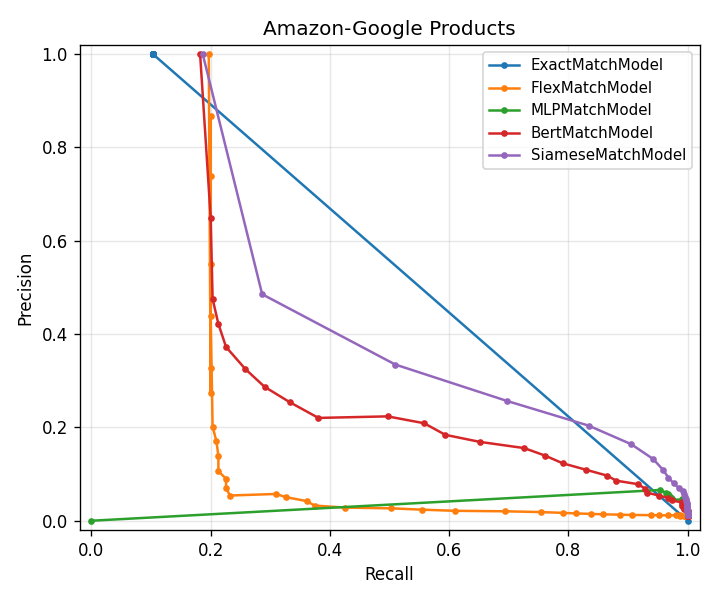
\includegraphics[width=\linewidth]{../docs/pr/pr_amazon-google.png}
\caption{Amazon-Google Products}
\end{subfigure}
\hfill
\begin{subfigure}[t]{0.48\textwidth}
\centering
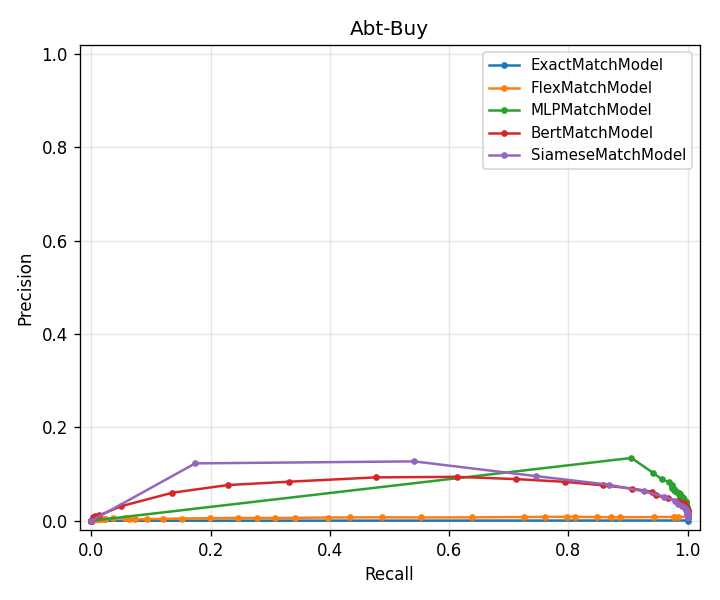
\includegraphics[width=\linewidth]{../docs/pr/pr_abt-buy.png}
\caption{Abt-Buy}
\end{subfigure}

\vspace{6pt}

\begin{subfigure}[t]{0.48\textwidth}
\centering
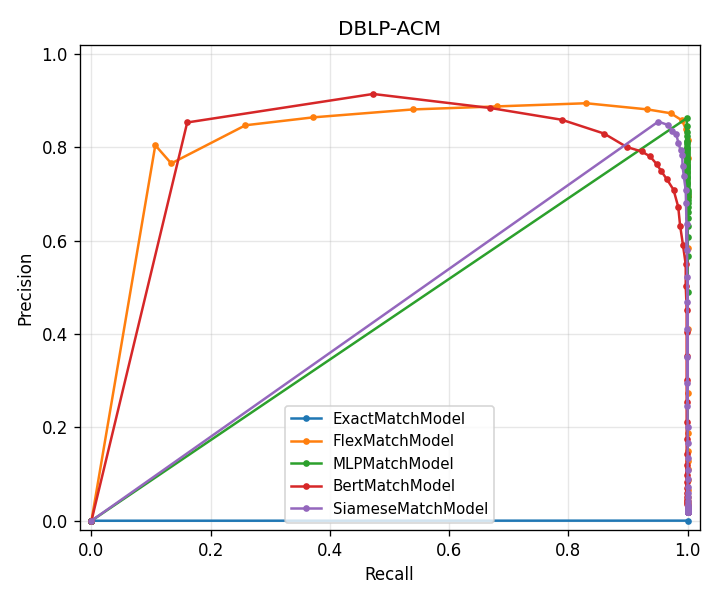
\includegraphics[width=\linewidth]{../docs/pr/pr_dblp-acm.png}
\caption{DBLP-ACM}
\end{subfigure}
\hfill
\begin{subfigure}[t]{0.48\textwidth}
\centering
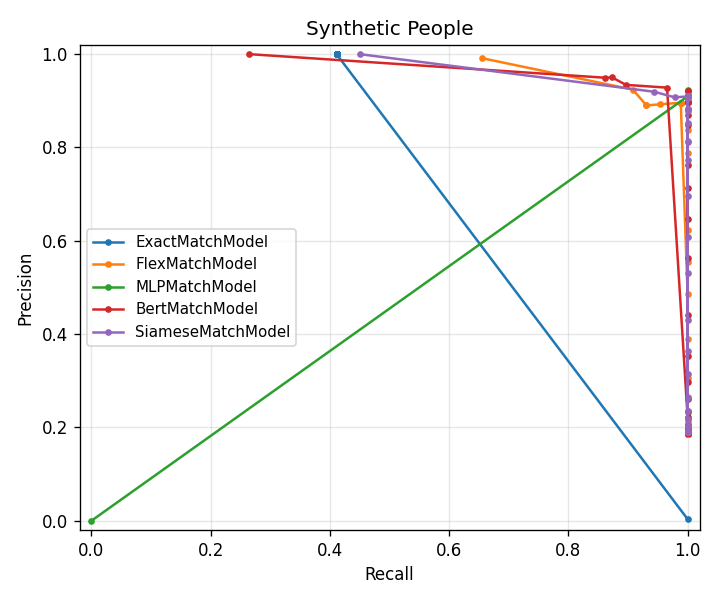
\includegraphics[width=\linewidth]{../docs/pr/pr_synthetic-people.png}
\caption{Synthetic People}
\end{subfigure}
\caption{Precision-recall curves across the four benchmark datasets.
Each curve is one model swept across thresholds 0 to 1 in steps of
0.02. ExactMatch collapses to a point because it produces a binary
score.}
\label{fig:pr}
\end{figure*}

\section{Discussion}
\label{sec:discussion}

The five-model design lets us examine where the methodological
progression of the field actually pays off and where it does not.
Four datasets surface four distinct patterns.

\subsection{Loose-text product catalogs reward fine-tuning (Amazon-Google)}

On Amazon-Google the MRR improves with model sophistication. ExactMatch
produces 0.13, the rule-based Flex produces 0.25, the supervised MLP
produces 0.40, the pretrained BERT produces 0.39, and the fine-tuned
Siamese produces 0.46. This is the pattern the literature would
predict for a free-text dataset in which the same product is described
in materially different language by the two sources. The fine-tuned
encoder benefits from having seen positive and negative pairs from the
dataset itself, and the resulting embedding geometry rewards
near-paraphrases of product descriptions even when the surface forms
diverge. The per-seed variance on Siamese (0.018) is small enough that
the seven-MRR-point lead over BERT is unlikely to be seed noise.

The classification F1 column tells a different story. ExactMatch wins
F1 at 0.187 because it produces few candidate pairs and those it
produces are uniformly correct (precision 1.0). The trained models all
score below F1 0.10 because their candidate sets are much larger and
the threshold of 0.5 admits too many false positives. This is a
calibration issue rather than a ranking failure, and the
precision-recall sweep in Figure \ref{fig:pr} shows that the encoder
models can recover useful F1 at higher thresholds.

\subsection{Cross-catalog text breaks BERT but not MLP (Abt-Buy)}

The Abt-Buy result is the most striking. The MLP achieves MRR 0.64,
well ahead of the fine-tuned Siamese at 0.53 and the pretrained BERT
at 0.41. This inverts the order on Amazon-Google. Three observations
help explain it. First, Abt-Buy is the smallest of the real-world
benchmarks (about 2200 records) and the supervision signal is
correspondingly thinner. The seed standard deviation for MLP (0.051)
is roughly three times what it was on Amazon-Google, suggesting that
pair sampling matters more when the underlying training set is
smaller. Second, Abt and Buy describe products in radically different
registers, with Abt offering long marketing-prose descriptions and
Buy offering terse listings. This kind of cross-domain language gap
is exactly the case that generic semantic similarity, as offered by
the pretrained sentence-transformer, fails to bridge. The MLP, by
contrast, learns on the labeled pairs which similarity dimensions
actually carry signal, and it can downweight the prose-versus-terse
mismatch in favor of correlations on name and price. Third, the
Siamese model does help over pretrained BERT (0.53 versus 0.41) but
does not catch up to MLP. We interpret this as evidence that on a
small, noisy benchmark, the encoder fine-tuning has too little
supervision to specialize the embedding geometry usefully.

The takeaway from Abt-Buy is that on this kind of cross-catalog
small-vocabulary corpus, engineered features plus a learned weighting
still beat pretrained encoders, with or without fine-tuning. This is
consistent with observations in the older line of supervised ER
research \citep{bilenko2003, cohen2003} but is not the conclusion a
casual reading of the deep-ER literature would predict.

\subsection{Saturated structured benchmark (DBLP-ACM)}

DBLP-ACM is widely understood to be near-saturated. The four trained
models all reach MRR 0.93 to 0.94, and the rank ordering they impose
on candidate matches is essentially identical. The classification F1
at the fixed 0.5 threshold separates the models, with the MLP at 0.86
and the others below 0.30. The MLP advantage comes from its calibrated
classifier head, which produces a usefully bimodal score distribution
at inference time, while the cosine-similarity models place too many
non-matching pairs above 0.5. This is a calibration issue rather than
a failure of ranking.

Ditto \citep{li2020} reports F1 0.989 on this dataset using its
labeled-pair protocol. Our MLP's F1 of 0.86 on the all-pairs candidate
set is lower because the protocol is harder, not because the model is
weaker.

\subsection{Synthetic perturbation favors engineered features (Synthetic People)}

The synthetic person corpus poses a different challenge. Close-match
pairs are produced by random one-character or one-field perturbations
that do not follow any systematic pattern. There is no semantic
relationship between a name with a leading character dropped and the
original name, in the sense that a pretrained language model would
have learned. The MLP wins F1 by a wide margin (0.95 versus 0.76 for
Siamese, 0.47 for Flex, and 0.33 for BERT). This is again consistent
with the Abt-Buy story. When the data-generating process is
character-noise rather than semantic-paraphrase, the signal lives in
specific string-similarity scores rather than in a learned embedding
geometry.

The MRR numbers on Synthetic People are also notably higher than they
would be on a full-data evaluation. This is because the held-out test
set excludes singletons, which by construction have no positive match
to find in the corpus, and which would otherwise dilute the MRR.

\subsection{Synthesis}

Across the four datasets a single message recurs. The choice of
methodological tier matters less than the alignment between the
method's inductive bias and the dataset's data-generating process.
Pretrained encoders excel when the dataset's matching relation is a
form of semantic paraphrase. Engineered feature classifiers excel when
the relation is a form of structured noise. Fine-tuning helps in the
former case but cannot rescue the latter from a fundamentally
mismatched representation.

This finding is consistent with the broader observation in machine
learning that strong inductive bias often beats general-purpose
representation when the dataset is small and the task is narrow.

\section{Comparison to Published Baselines}
\label{sec:baselines}

For ceiling reference we compare the best F1 in our protocol against
the F1 reported by two strong deep-ER systems on the same datasets.
Table \ref{tab:baselines} reports these numbers.

\begin{table}[t]
\centering
\caption{F1 reported on these datasets by two strong deep-ER systems,
compared to this package's best F1 at threshold 0.5.}
\label{tab:baselines}
\small
\begin{tabular}{lccc}
\toprule
Dataset & DeepMatcher & Ditto & This work \\
\midrule
Amazon-Google & 0.694 & 0.751 & 0.187 (Exact) \\
Abt-Buy       & 0.628 & 0.892 & 0.092 (MLP) \\
DBLP-ACM      & 0.984 & 0.989 & 0.855 (MLP) \\
\bottomrule
\end{tabular}
\end{table}

DeepMatcher numbers are from \citet{mudgal2018} Table 4 (Hybrid
model). Ditto numbers are from \citet{li2020}. The Magellan baseline
of \citet{konda2016} is not directly comparable because the underlying
\texttt{py\_entitymatching} library does not install on Python 3.10 or
above at the time of writing.

These comparisons require a critical caveat. DeepMatcher and Ditto
both report F1 on a labeled-pair test set, that is, a balanced set of
positive and negative pairs sampled from the perfect mapping. We
report F1 on the all-pairs candidate set produced by blocking, which
is much larger and includes many more easy negatives. The two
quantities measure different things. The labeled-pair F1 asks ``given
a pair, is it a match,'' while the all-pairs F1 asks ``of all
candidates this model produced, how many of the predicted matches
were correct.'' A meaningful direct comparison would require
re-running DeepMatcher and Ditto under our protocol, which we have not
done. We treat the cited numbers as a ceiling reference rather than a
head-to-head bar.

Within our protocol, DBLP-ACM still has headroom for the MLP (F1
0.855 versus the published 0.989). Amazon-Google and Abt-Buy retain
much more headroom, with the gap to
the published numbers traceable to a combination of blocking recall,
threshold calibration, and the protocol mismatch.

\section{Limitations}
\label{sec:limitations}

The Magellan baseline was not re-run because
\texttt{py\_entitymatching} does not install on the Python 3.10+
environment in which the rest of the package runs. The DeepMatcher
and Ditto numbers cited in Section \ref{sec:baselines} are from those
papers' published evaluations under their own protocols, which use
labeled-pair test sets rather than the all-pairs candidate set we use
here. The two cannot be directly compared.

The fixed threshold of 0.5 for the F1 column is the dominant source
of the spread between MRR (where models cluster) and F1 (where
calibration separates them). A more decisive comparison would tune
the threshold per model on a held-out validation set. The
precision-recall sweep in Figure \ref{fig:pr} substitutes for that to
some extent.

The synthetic person dataset was generated by the package itself.
While the underlying perturbation rules are documented and
reproducible, the resulting corpus is not standardized and its
results should be interpreted as a controlled case study rather than
a benchmark.

The held-out group split partitions groups 70/30 with a single random
seed. A more careful evaluation would average across multiple splits.
The current results report multi-seed variance for the stochastic
models but not multi-split variance for the deterministic models.

\section{Reproducibility}
\label{sec:reproducibility}

The package, datasets, and trained model artifacts are available at
the GitHub repository linked from the Zenodo record. The full results
in this paper can be reproduced from a fresh checkout with:

\begin{verbatim}
git clone https://github.com/johnnysaldana/matchify.git
cd matchify
python3.12 -m venv .venv
source .venv/bin/activate
make install-deep
make bench
\end{verbatim}

The \texttt{make bench} target runs the full
five-models-on-four-datasets sweep with the held-out split, three
seeds, and the precision-recall threshold sweep. Output is written to
\texttt{output.html} for the side-by-side prediction tables and to
\texttt{docs/pr/} for the precision-recall curves. The benchmark takes
approximately three hours on an Apple M-series MacBook (mostly
Siamese fine-tuning across three seeds on each dataset).

The package archive is registered with Zenodo for citation. See
\texttt{CITATION.cff} for the canonical citation.

\section*{Acknowledgements}

This work was carried out under the supervision of Dr. Tom Lippincott
of the Center for Language and Speech Processing at Johns Hopkins
University, in the course EN.601.507 Applied Entity Resolution and
Deduplication, Spring 2023. The literature reading list and the
methodological framing draw on the textbooks of \citet{christen2012}
and \citet{papadakis2021} and on the papers collected during the
course.

\bibliographystyle{plainnat}
\bibliography{references}

\end{document}
